\section{moeo\-Objective\-Objective\-Vector\-Comparator$<$ Objective\-Vector $>$ Class Template Reference}
\label{classmoeoObjectiveObjectiveVectorComparator}\index{moeoObjectiveObjectiveVectorComparator@{moeoObjectiveObjectiveVectorComparator}}
Functor allowing to compare two objective vectors according to their first objective value, then their second, and so on.  


{\tt \#include $<$moeo\-Objective\-Objective\-Vector\-Comparator.h$>$}

Inheritance diagram for moeo\-Objective\-Objective\-Vector\-Comparator$<$ Objective\-Vector $>$::\begin{figure}[H]
\begin{center}
\leavevmode
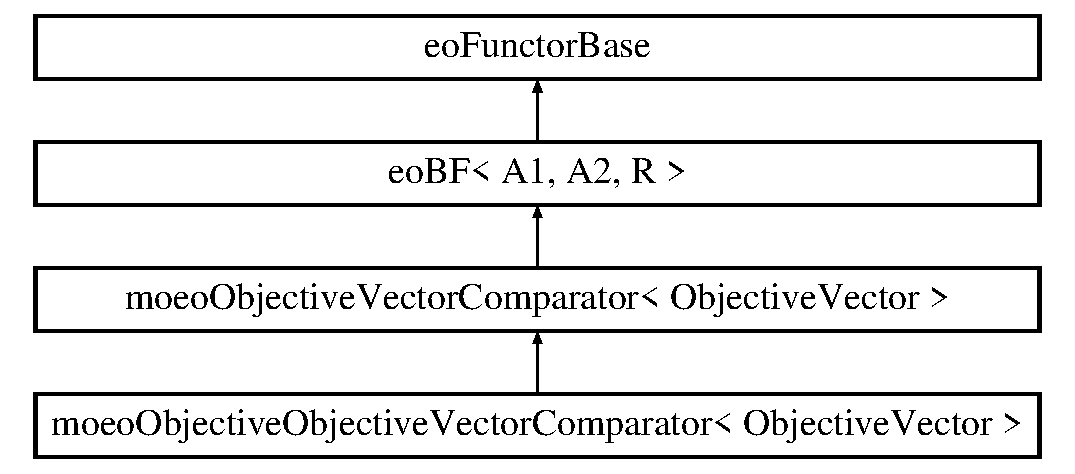
\includegraphics[height=4cm]{classmoeoObjectiveObjectiveVectorComparator}
\end{center}
\end{figure}
\subsection*{Public Member Functions}
\begin{CompactItemize}
\item 
const bool \bf{operator()} (const Objective\-Vector \&\_\-objective\-Vector1, const Objective\-Vector \&\_\-objective\-Vector2)
\begin{CompactList}\small\item\em Returns true if \_\-objective\-Vector1 $<$ \_\-objective\-Vector2 on the first objective, then on the second, and so on. \item\end{CompactList}\end{CompactItemize}


\subsection{Detailed Description}
\subsubsection*{template$<$class Objective\-Vector$>$ class moeo\-Objective\-Objective\-Vector\-Comparator$<$ Objective\-Vector $>$}

Functor allowing to compare two objective vectors according to their first objective value, then their second, and so on. 



Definition at line 22 of file moeo\-Objective\-Objective\-Vector\-Comparator.h.

\subsection{Member Function Documentation}
\index{moeoObjectiveObjectiveVectorComparator@{moeo\-Objective\-Objective\-Vector\-Comparator}!operator()@{operator()}}
\index{operator()@{operator()}!moeoObjectiveObjectiveVectorComparator@{moeo\-Objective\-Objective\-Vector\-Comparator}}
\subsubsection{\setlength{\rightskip}{0pt plus 5cm}template$<$class Objective\-Vector$>$ const bool \bf{moeo\-Objective\-Objective\-Vector\-Comparator}$<$ Objective\-Vector $>$::operator() (const Objective\-Vector \& {\em \_\-objective\-Vector1}, const Objective\-Vector \& {\em \_\-objective\-Vector2})\hspace{0.3cm}{\tt  [inline]}}\label{classmoeoObjectiveObjectiveVectorComparator_bc3c97b380e87107e92f52843a7f9303}


Returns true if \_\-objective\-Vector1 $<$ \_\-objective\-Vector2 on the first objective, then on the second, and so on. 

\begin{Desc}
\item[Parameters:]
\begin{description}
\item[{\em \_\-objective\-Vector1}]the first objective vector \item[{\em \_\-objective\-Vector2}]the second objective vector \end{description}
\end{Desc}


Definition at line 31 of file moeo\-Objective\-Objective\-Vector\-Comparator.h.

The documentation for this class was generated from the following file:\begin{CompactItemize}
\item 
moeo\-Objective\-Objective\-Vector\-Comparator.h\end{CompactItemize}
